\documentclass[12pt]{amsart}
%prepared in AMSLaTeX, under LaTeX2e
\addtolength{\oddsidemargin}{-.5in}
\addtolength{\evensidemargin}{-.5in}
\addtolength{\topmargin}{-0.5in}
\addtolength{\textwidth}{1.1in}
\addtolength{\textheight}{1.0in}
\newcommand{\normalspacing}{\renewcommand{\baselinestretch}{1.05}
        \tiny\normalsize}

\newtheorem*{thm}{Theorem}
\newtheorem*{defn}{Definition}
\newtheorem*{example}{Example}
\newtheorem*{problem}{Problem}
\newtheorem*{remark}{Remark}

\usepackage{amssymb,fancyvrb,xspace}
\usepackage{palatino}

\usepackage[final]{graphicx}

\usepackage{tikz}
\usetikzlibrary{shapes,arrows,arrows.meta}


\usepackage[pdftex, colorlinks=true, plainpages=false, linkcolor=black, citecolor=red, urlcolor=red]{hyperref}

% macros
\newcommand{\ba}{\mathbf{a}}
\newcommand{\bb}{\mathbf{b}}
\newcommand{\bn}{\mathbf{n}}
\newcommand{\br}{\mathbf{r}}
\newcommand{\bu}{\mathbf{u}}
\newcommand{\bv}{\mathbf{v}}
\newcommand{\bx}{\mathbf{x}}
\newcommand{\by}{\mathbf{y}}

\newcommand{\bT}{\mathbf{T}}

\newcommand{\CC}{\mathbb{C}}
\newcommand{\Div}{\nabla\cdot}
\newcommand{\eps}{\epsilon}
\newcommand{\grad}{\nabla}
\newcommand{\ZZ}{\mathbb{Z}}
\newcommand{\ip}[2]{\ensuremath{\left<#1,#2\right>}}
\newcommand{\lam}{\lambda}
\newcommand{\lap}{\triangle}
\newcommand{\RR}{\mathbb{R}}

\newcommand{\prob}[1]{\bigskip\noindent\large\textbf{#1}.\,\normalsize }
\newcommand{\ppart}[1]{\textbf{(#1)}\,\, }
\newcommand{\epart}[1]{\medskip\noindent\textbf{(#1)}\,\, }

\newcommand{\pts}[1]{\scriptsize [#1 points] \normalsize}

\newcommand{\Matlab}{\textsc{Matlab}\xspace}
\newcommand{\Python}{\textsc{Python}\xspace}
\newcommand{\Julia}{\textsc{Julia}\xspace}


\begin{document}
\scriptsize \noindent Math 661 Optimization \, (Bueler) \hfill  31 October, 2022
\normalsize\bigskip
\normalspacing

\Large\centerline{\textbf{About your project}}
\normalsize

\bigskip\medskip
\thispagestyle{empty}
\normalspacing

\subsection*{Goal}  The goal of the Math 661 project is for you to focus on topics of particular interest, and become more familiar with certain optimization problems and algorithms than is possible with the brief coverage typical of the rest of the course.

\subsection*{Expectations}  Your project may be application-driven (\emph{choose the problem(s) first}) or algorithm-driven (\emph{choose the algorithm(s) first}).  However, all projects must include both a specific optimization problem and a specific optimization algorithm.  You will implement at least one algorithm, i.e.~by a code you write in \Matlab/\Python/ \Julia/etc., and then apply your code to at least one example problem.

Both numerical computation and mathematical analysis are required.  For the latter you will analyze the problem(s) and algorithm(s) using theory from the textbook\footnote{Griva, Nash, and Sofer, \emph{Linear and Nonlinear Optimization}, 2nd ed., SIAM Press 2009.} and/or from other references.  Once your code is running you should provide some empirical (numerical experimentation) evidence regarding the error and/or performance of your algorithm(s).

Analysis is important as it shows you have absorbed ideas from the course, and because it distinquishes between algorithms.  Numerical evidence shows that you understood the algorithm well enough to implement it correctly.

The problem(s) you choose must be in the following form:
\begin{equation}
\min_{x\in \RR^n} f(x) \quad \text{subject to} \quad \begin{matrix}
                                                      g_i(x) = 0, & i \in \mathcal{E}, \\
                                                      g_i(x) \ge 0, & i \in \mathcal{I},
                                                      \end{matrix}  \label{genform}
\end{equation}
(Of course you may replace $\min$ with $\max$.)  If your project is algorithm-driven then you must identify which such problems are solved by your algorithms(s).

Form \eqref{genform} describes a very large class of problems.  Your problem(s) must be finite-dimensional, but they may arise from an infinite-dimensional source.  The problem(s) must be well-enough understood to allow you to both precisely identify the objective function $f(x)$ and to precisely identify a feasible set $S$ defined by finitely-many equality and inequality constraints $g_i(x)$.  It is o.k.~if there are no constraints, with $\mathcal{E}$ and $\mathcal{I}$ as empty sets, but I may provide feedback on your Part I proposal which suggests you consider a constrained form of your problem.


\subsection*{Due dates}  There are two due dates for the project:

\subsubsection*{Part I = project proposal:}  \textbf{Part I is due Friday 11 November at the start of class.}

There are no format requirements for this part, but it must be \textbf{two pages or less}.

The proposal should precisely say what problem(s) or algorithm(s) you will address.  If application-driven it should explain \emph{briefly} where the optimization problem(s) came from.  In any case it should briefly motivate your proposed choice(s) of algorithm(s).  Several quality references are \emph{expected}; online references are o.k.~though many informal online documents are of low quality.  Please make specific references to our textbook when that is appropriate.  Finally, your proposal should talk though what the complete project will contain, to the degree possible.

Spending at least a few hours on thinking and research at this stage can be very effective, but I suggest that you spend at most 6 hours on Part I.

\subsubsection*{Part II = actual project:}  \textbf{The completed project is due Monday 12 December at 5pm.}

It should have the format as shown below on page 4.  Please use the indicated section headings!  The total length \textbf{must be 20 pages or less}; I will not accept longer projects.  The total time spent on the whole project should be at most 25 hours.

The format expectations can be met by using the \LaTeX\xspace template posted online at \href{https://bueler.github.io/opt/projects.html}{\texttt{bueler.github.io/opt/projects.html}}, but you do not have to use \LaTeX.


\subsection*{Choosing a topic}  One of my jobs will be to help you choose problem(s) and algorithm(s) so that your project has reasonable difficulty.  The bigger the scope the easier it is to get lost in the application, the algorithmic details, or difficulties with programming/debugging/analysis.  Your Part I proposal allows me to give good feedback on the topic, perhaps a gentle nudge in the direction of a nice variation in topic, or a different analysis to consider, or that you bite off less, and etc.

You may \textbf{not} choose a topic which will be adequately covered in lecture.  For example, the basic simplex method is not a good topic.  However, continuing the example, implementations of the simplex method which respect sparsity, a topic we do not cover, would be a great choice (Chapter 7).  Similarly, the classical Newton method is not a good subject, but comparing quasi-Newton methods beyond BFGS, or line search methods beyond backtracking, or trust region methods, would all be good choices (Chapters 11 and 12).  Finally, there are many constrained optimization algorithms we will not get to, especially Chapters 8, 10, and 16. 

Here are three approaches to choosing a topic if you don't already have one:

\subsubsection*{Approach 1: Inspiration from the Wikipedia page on mathematical optimization}

See the ``Major subfields,'' ``Computational \dots techniques'', and ``Applications'' sections.

   \centerline{\href{https://en.wikipedia.org/wiki/Mathematical_optimization}{\texttt{en.wikipedia.org/wiki/Mathematical\_optimization}}}

\subsubsection*{Approach 2: Investigate skipped material from the textbook}  Consider section(s) that you find interesting and which we did not cover.  However, don't just choose a section at random; the above Wikipedia page is better for starting from scratch.

\subsubsection*{Approach 3: A topic related to your thesis (if you have one)}  Please talk to your thesis advisor.  It is reasonable to ask ``are there optimization problems related to my expected thesis''?  Often these are parameter fitting, inverse modeling, or optimal design problems.  On the other hand there may be significant algorithms which arise in your field of interest.  There may be a paper to read about optimization in your field.  Please \textbf{do not} cover territory comparable to your whole thesis; instead extract a little part and do it carefully.  You should also talk to me, but it may take a while for me to understand the context of your problem.


\newpage
\subsection*{Structure of the project}  Here is a rough flow-chart.  It aligns well with the section headings on the next page.

\bigskip

% Define block styles
\tikzstyle{decision} = [diamond, draw,
    text width=4.5em, text centered, node distance=3cm, inner sep=0pt]
\tikzstyle{block} = [rectangle, draw,
    text width=9em, text badly centered, rounded corners, minimum height=4em]
\tikzstyle{bigblock} = [rectangle, draw,
    text width=24em, text badly centered, rounded corners, minimum height=4em]
\tikzstyle{line} = [draw, -{Latex[length=3mm, width=2mm]}]

\begin{center}
\begin{tikzpicture}[node distance=2.4cm, auto, font=\small]
    % decide
    \node [decision] (decide) {your project is driven by};

    % algorithm sequence
    \node [block, below left of=decide, node distance=4cm] (introalg) {introduce algorithm(s)};
    \path [line] (decide.west) -- node [near start, left, yshift=4mm] {\textbf{algorithm}} (introalg.north);
    \node [block, below of=introalg] (algpseudo) {give pseudocode(s)};
    \path [line] (introalg) -- (algpseudo);
    \node [block, below of=algpseudo] (algexamples) {propose at least one example problem for testing};
    \path [line] (algpseudo) -- (algexamples);

    % application sequence
    \node [block, below right of=decide, node distance=4cm] (introapp) {introduce application(s)};
    \path [line] (decide.east) -- node [near start] {\textbf{application}} (introapp.north);
    \node [block, below of=introapp] (appexamples) {describe at least one example problem};
    \path [line] (introapp) -- (appexamples);
    \node [block, below of=appexamples] (appcompare) {describe at least one algorithm; give pseudocodes};
    \path [line] (appexamples) -- (appcompare);

    % merge and continue
    \node [block, below of=decide, node distance=10.5cm] (implement) {implement algorithms in \Matlab, \Python, \Julia, \dots};
    \path [line] (algexamples) -- (implement);
    \path [line] (appcompare) -- (implement);
    \node [block, below of=implement] (results) {demonstrate runs on example(s); show results};
    \path [line] (implement) -- (results);
    \node [bigblock, below of=results] (analysis) {analysis: \begin{itemize}
       \item convergence: e.g.~state theorems; compare rates
       \item performance: e.g.~count operations; show timing
       \end{itemize}     };
    \path [line] (results) -- (analysis);
    \node [block, below of=analysis] (conclude) {what you would do next? conclude};
    \path [line] (analysis) -- (conclude);
\end{tikzpicture}
\end{center}

\clearpage
\newpage

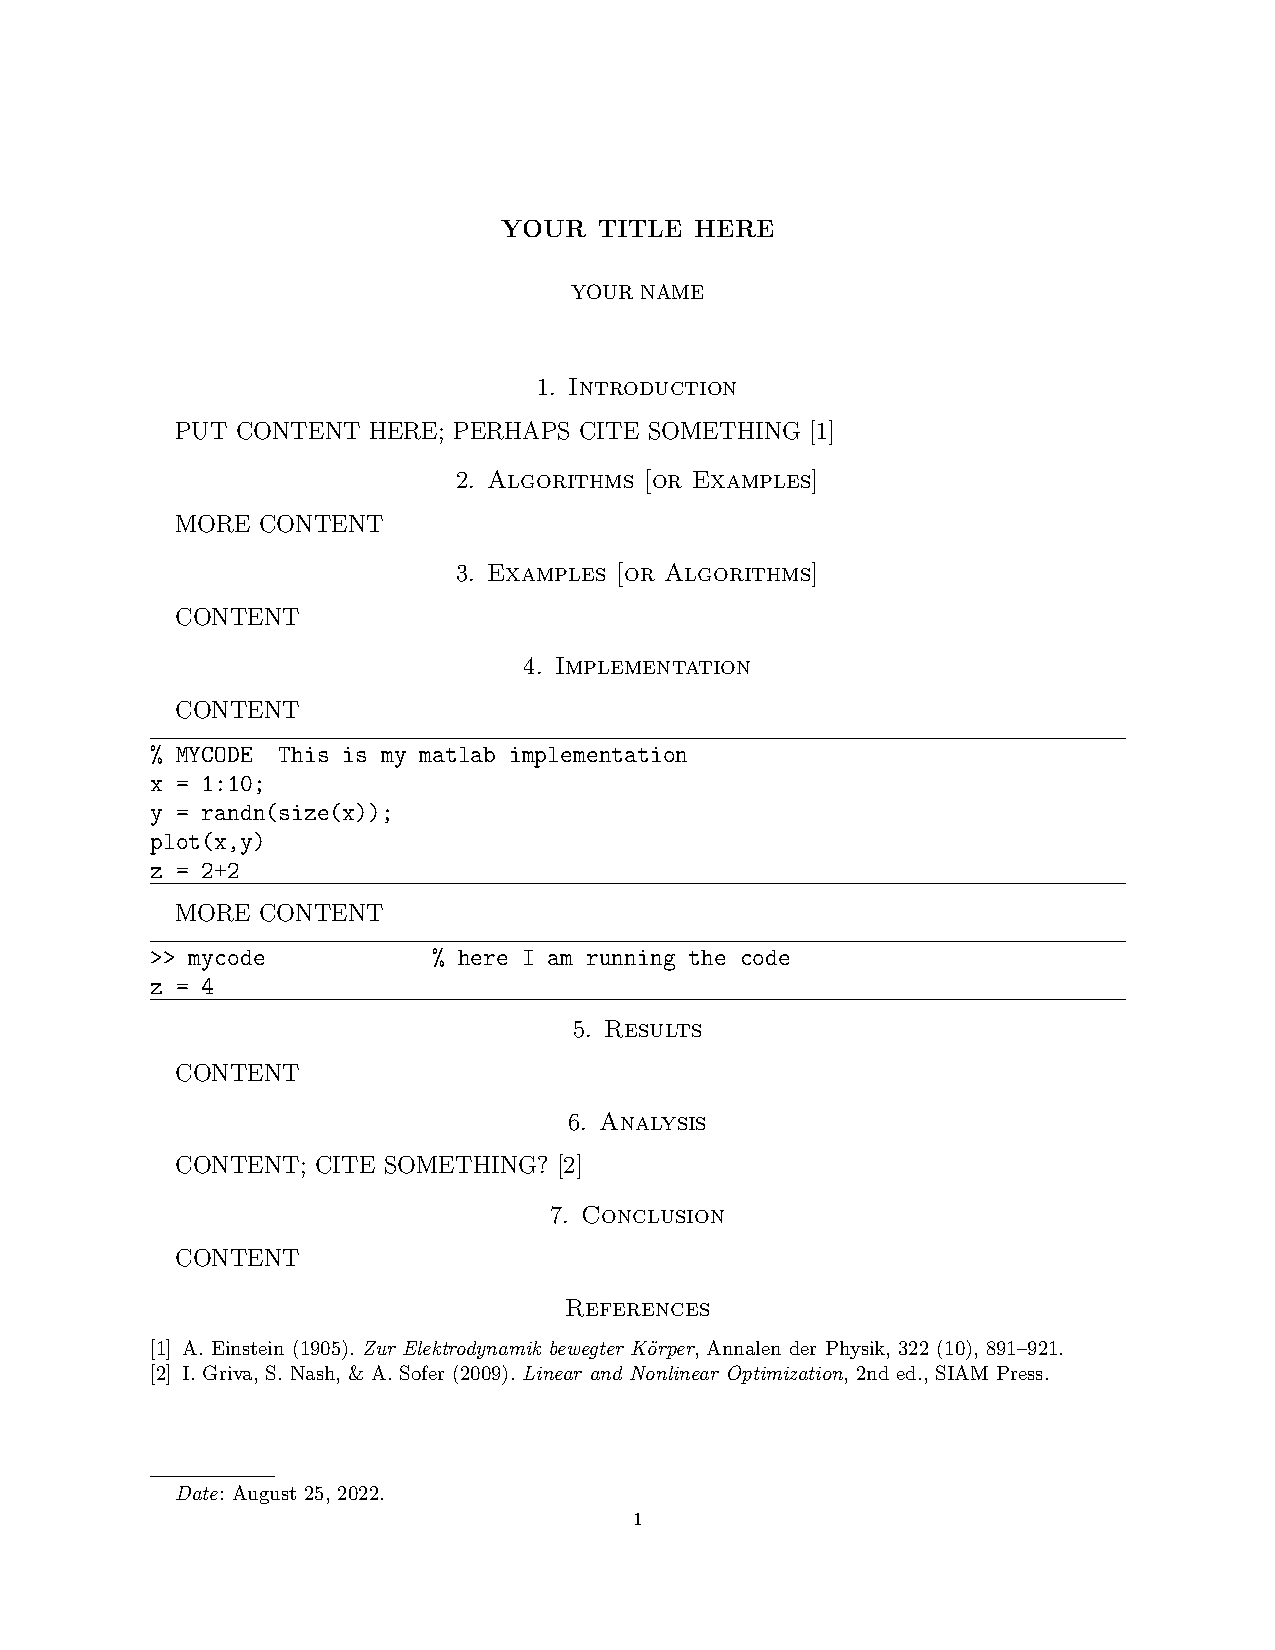
\includegraphics[height=\textheight]{blank.pdf}
\end{document}
